\section{Auswertung}
\label{sec:Auswertung}
\subsection{Messung der Topografie einer Mikrostruktur}
Im Verlauf der ersten Versuchsreihe werden verschiedene Strukturformen auf einer Mikrostrukturprobe betrachtet.
Mittels des AFM-Aufbaus werden von den drei vorhandenen Strukturen AFM-Bilder aufgenommen.
Es wird jeweils eine $(20 \times 20) \, \upmu \text{m}^2$ gro{\ss}e Fl\"ache vermessen.
In den Abbildungen \ref{abb:kreis} bis \ref{abb:streif} sind diese Bilder zu sehen.
Abgebildet sind nicht nur die AFM-Aufnahmen, sondern auch die Strecken, welche vermessen wurden.
\begin{figure}[H]
\centering
	\begin{subfigure}[t]{0.45\textwidth}
	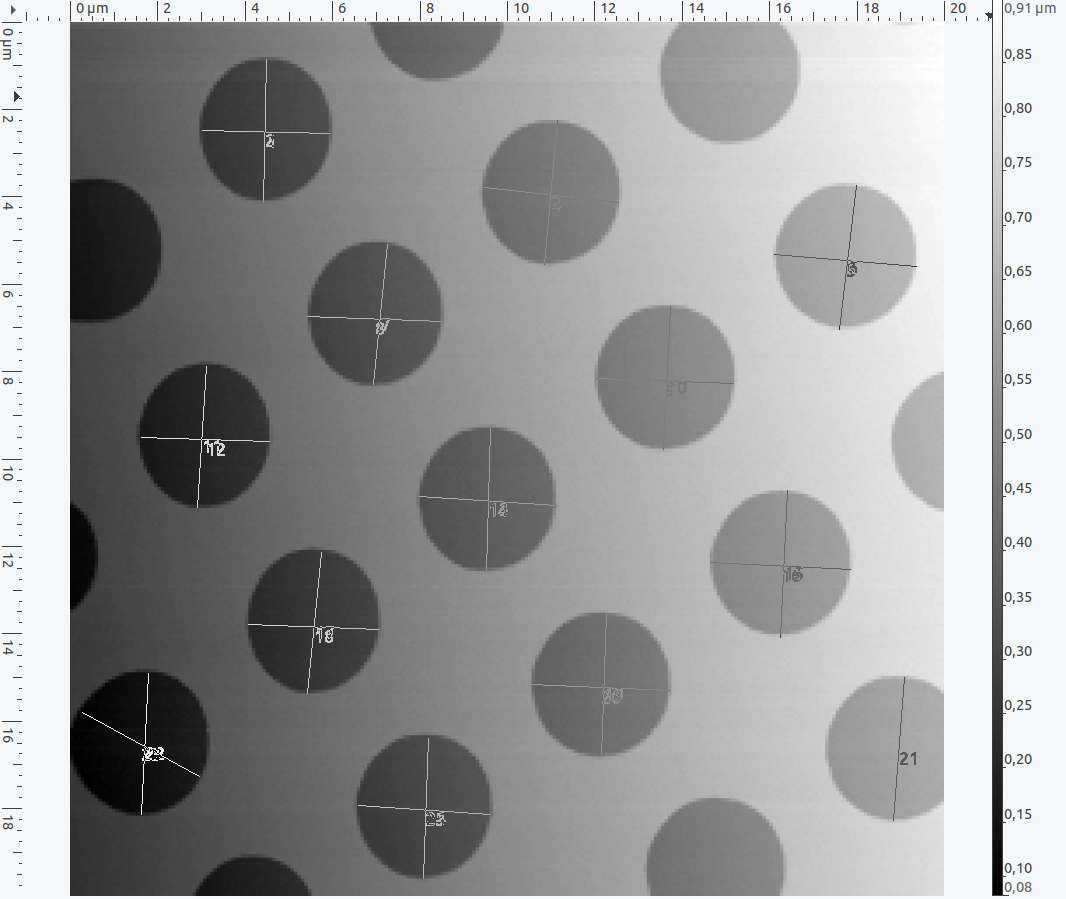
\includegraphics[width=\textwidth]{AFM_auswertung/Kreis_durch_vor.png}
	\caption{Vermessung des Kreisdurchmessers.}
	\label{abb:kreisa}
	\end{subfigure}
	~
	\begin{subfigure}[t]{0.45\textwidth}
	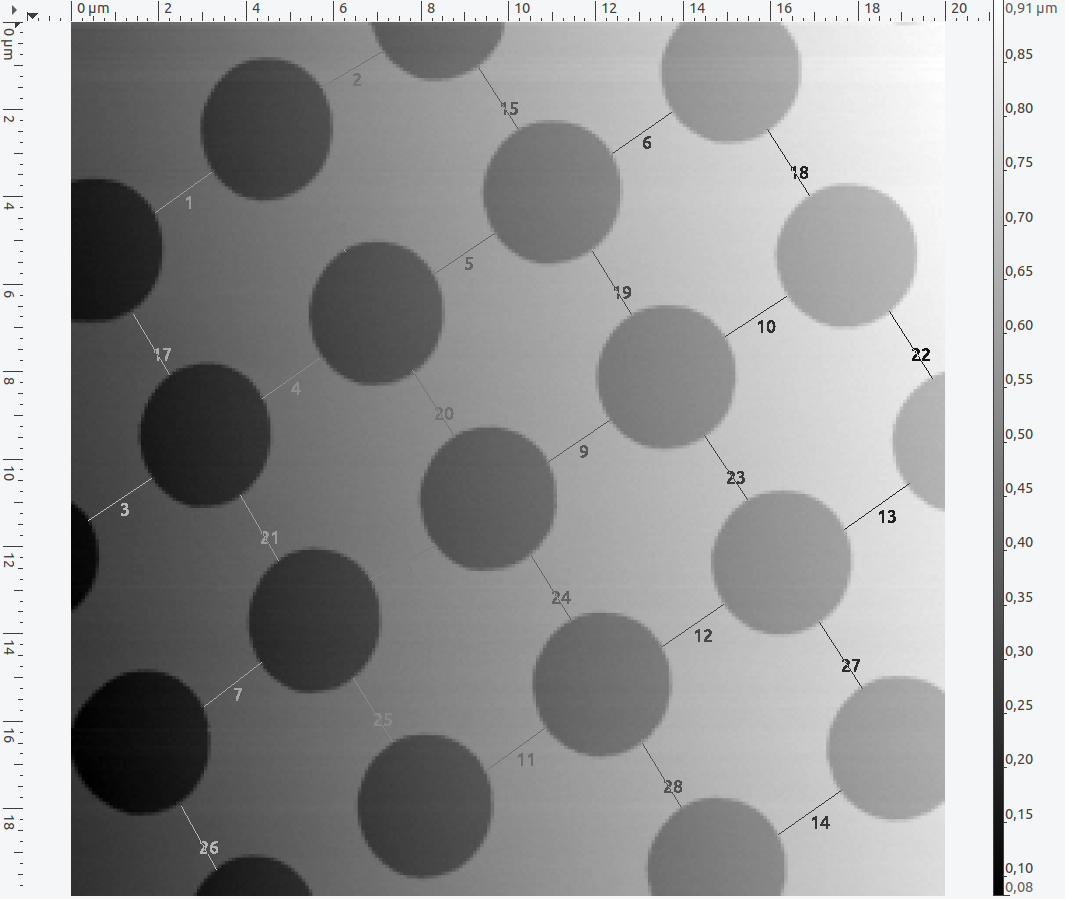
\includegraphics[width=\textwidth]{AFM_auswertung/Kreis_abs_vor.png}
	\caption{Bestimmung des Abstands zwischen den Kreisen.}
	\label{abb:kreisb}
	\end{subfigure}
\caption{Vermessung der Kreisstruktur auf der Mikrostrukturprobe. Aufgenommen wurde eine Fl\"ache der Gr\"o{\ss}e von $(20 \times 20) \, \upmu \text{m}^2$. Zur Vermessung der jeweiligen Strecken wurde das 'distance and direction-Tool' des Auswertungsprogram Gwyddion verwendet.}
\label{abb:kreis}
\end{figure}
\begin{figure}[H]
\centering
	\begin{subfigure}[t]{0.45\textwidth}
	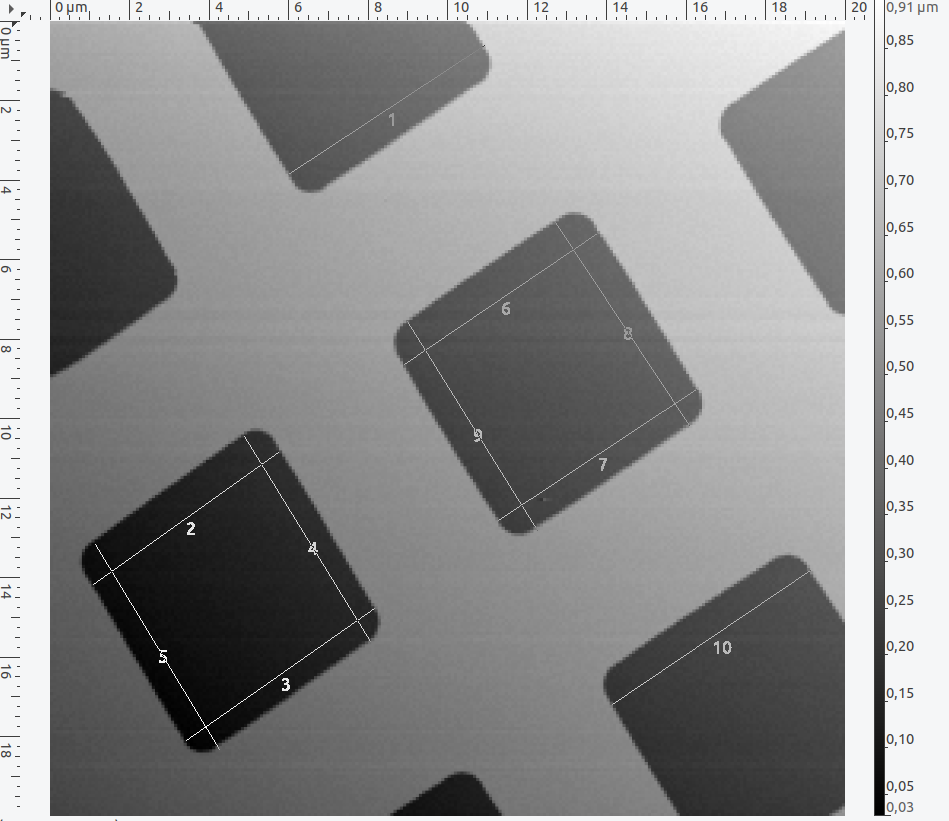
\includegraphics[width=\textwidth]{AFM_auswertung/quad_durch_vor.png}
	\caption{Vermessung der Quadratgr\"o{\ss}e.}
	\label{abb:quada}
	\end{subfigure}
	~
	\begin{subfigure}[t]{0.45\textwidth}
	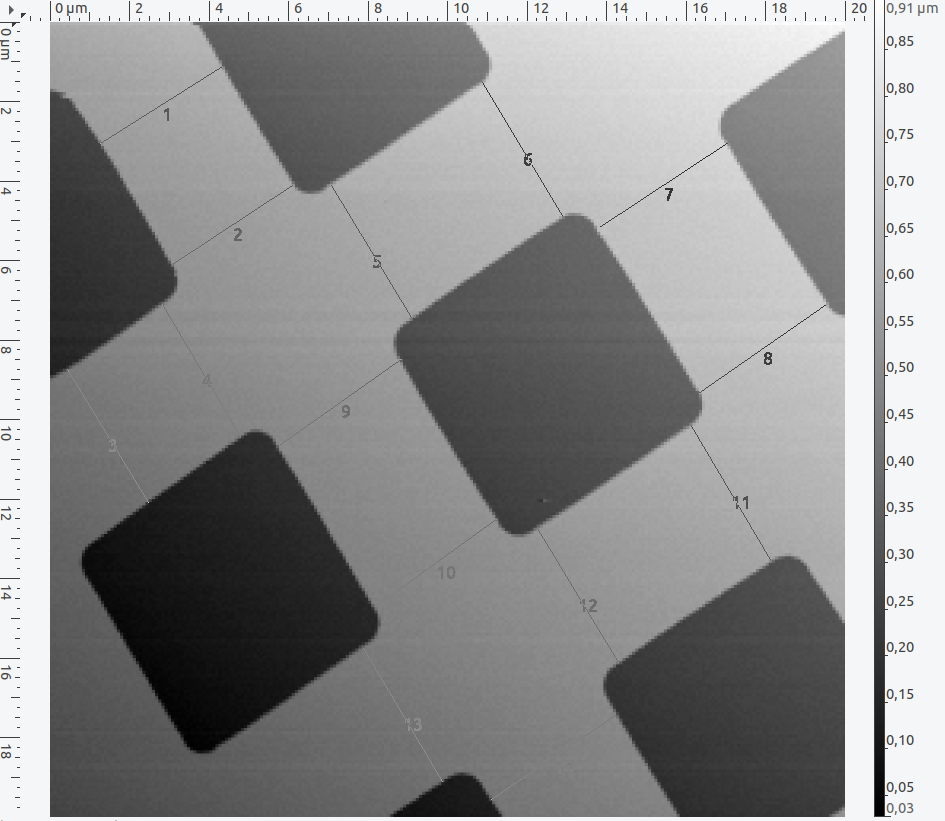
\includegraphics[width=\textwidth]{AFM_auswertung/quad_abb_vor.png}
	\caption{Bestimmung des Abstands zwischen den Quadraten.}
	\label{abb:quadb}
	\end{subfigure}
\caption{Vermessung der Quadratstruktur auf der Mikrostrukturprobe. Aufgenommen wurde eine Fl\"ache der Gr\"o{\ss}e von $(20 \times 20) \, \upmu \text{m}^2$. Zur Vermessung der jeweiligen Strecken wurde das 'distance and direction-Tool' des Auswertungsprogram Gwyddion verwendet.}
\label{abb:quad}
\end{figure}
%
\begin{figure}[H]
\centering
	\begin{subfigure}[t]{0.45\textwidth}
	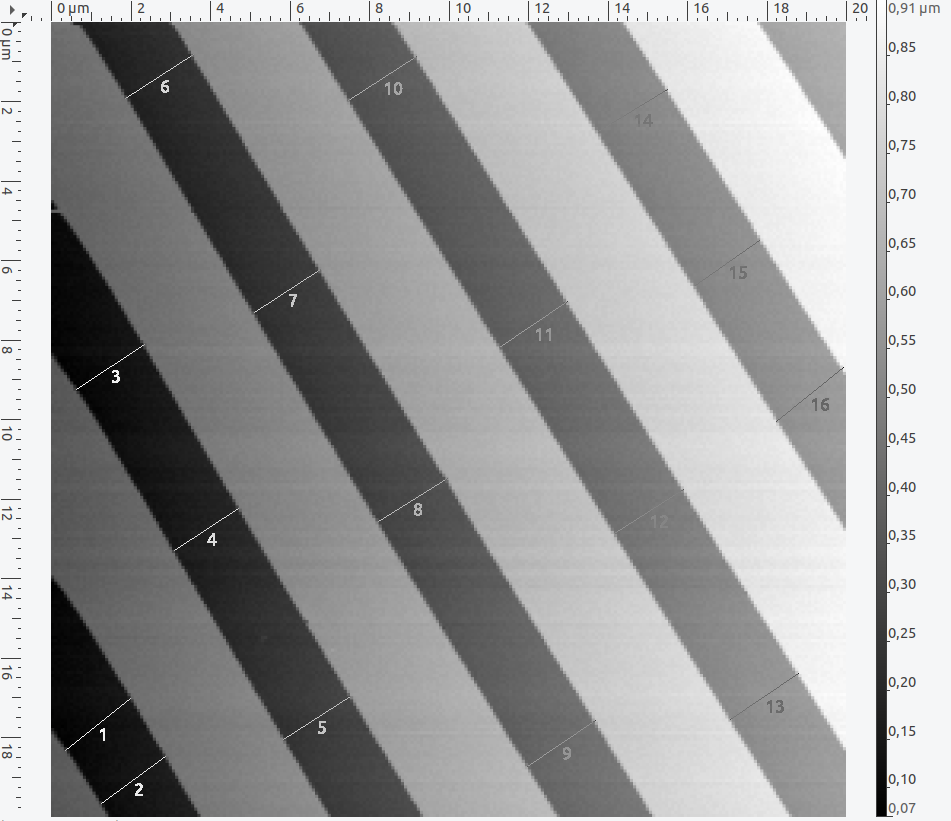
\includegraphics[width=\textwidth]{AFM_auswertung/streif_durch_vor.png}
	\caption{Vermessung der Streifenbreite.}
	\label{abb:streifa}
	\end{subfigure}
	~
	\begin{subfigure}[t]{0.45\textwidth}
	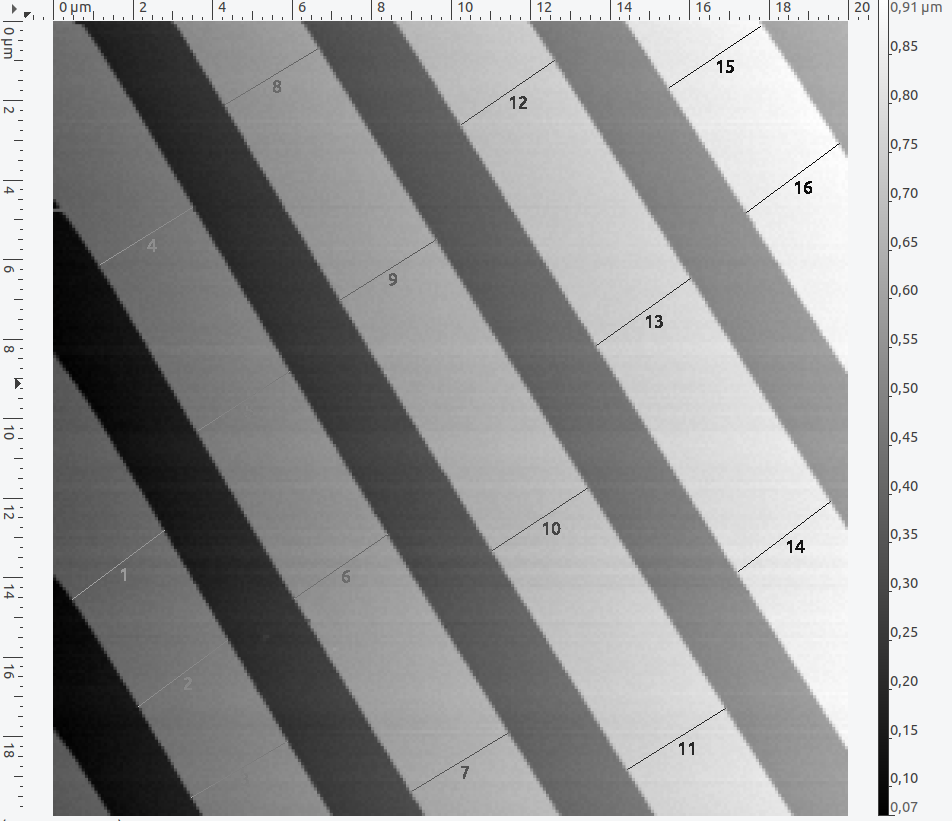
\includegraphics[width=\textwidth]{AFM_auswertung/streif_abb_vor.png}
	\caption{Vermessung des Abstands zwischen zwei Streifen.}
	\label{abb:streifb}
	\end{subfigure}
\caption{Vermessung der Streifen auf der Mikrostrukturprobe. Aufgenommen wurde eine Fl\"ache der Gr\"o{\ss}e von $(20 \times 20) \, \upmu \text{m}^2$. Zur Vermessung der jeweiligen Strecken wurde das 'distance and direction-Tool' des Auswertungsprogram Gwyddion verwendet.}
\label{abb:streif}
\end{figure}
%
Die vermessenen Strecken sind in den einzelnen Bildern mit Nummern versehen und wurden mit Hilfe des Auswertungsprogram Gwyddion erstellt.
In Tabelle \ref{tab:auf1} sind die Mittelwerte der aufgenommenen Werte aufgelistet.
Die experimentell bestimmten Daten werden mit den Strukturabst\"anden aus dem Datenblatt \cite{anleitung} verglichen.
Diese sind, genau wie die zugeh\"ohrigen Abweichungen, auch in Tabelle \ref{tab:auf1} festgehalten.
\begin{table}
	\centering
	\caption{Messwerte der Mikrostrukturprobe. Aufgelistet sind die gemittelten Werte der vermessenen Strecken und Abst\"ande. Der Strukturabstand ergibt sich aus der Summe von Gr\"o{\ss}e und Abstand der Mikrostruktur.}
\begin{tabular}{|r|ccc|}
	\hline
	{} & {Kreis} & {Quadrat} & {Streifen} \\
	\hline
	Größe / $\upmu \text{m}$ & $3,18 \pm 0,10$ & $5,96 \pm 0,12$ & $2,04 \pm 0,04$ \\
	Abstand / $\upmu \text{m}$ & $1,69 \pm 0,05$ & $3,84 \pm 0,09$ & $2,83 \pm 0,06$ \\
	Strukturabstand / $\upmu \text{m}$ & $4,87 \pm 0,11$ & $ 9,80 \pm 0,15$ & $4,87 \pm 0,07$ \\
	Strukturabstand theo. / $\upmu \text{m}$ & 5 & 10 & 5 \\
	Abweichung / \%	& 2,7 & 2,03 & 2,62 \\
	\hline
\end{tabular}
\label{tab:auf1}
\end{table}


\subsection{Topographie einer CD, DVD und Blu-ray}
Im zweiten Teil des Versuches wird die Oberfl\"ache von drei unterschiedlichen Speichermedien, eine CD, eine DVD und eine Blu-ray, mit dem AFM untersucht.
Bevor die aufgenommenen Bilder und Daten mit Gwyddion ausgewertet werden, werden die Bilder gegl\"attet.
Hierf\"ur werden Bearbeitungstools von Gwyddion verwendet, welche den Hintergrund entfernen und einzelne Zeilen mit verschiedenen Methoden ausrichten.
In Abbildung \ref{abb:3d} sind die bearbeiteten 3D-AFM-Bilder der drei unterschiedliche Speichermedien zu sehen.
\begin{figure}[H]
\centering
	\begin{subfigure}[t]{0.5\textwidth}
	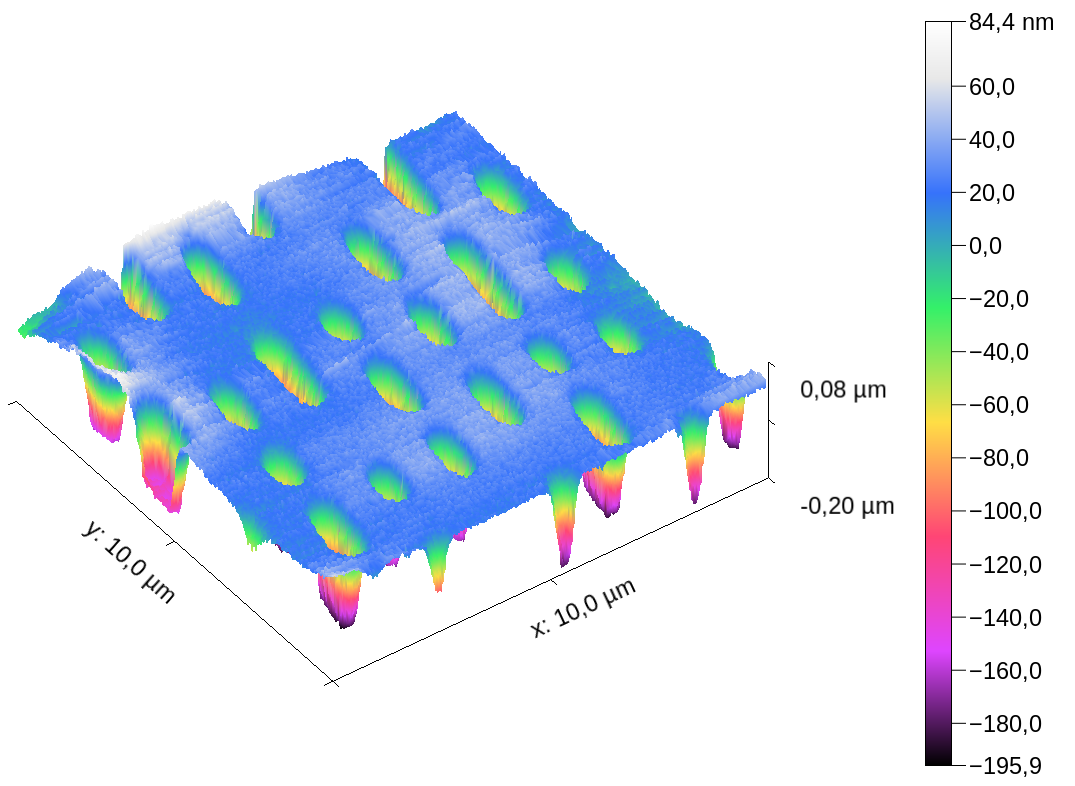
\includegraphics[width=\textwidth]{AFM_auswertung/cd_3D.png}
	\caption{3D-AFM-Bild der CD-Oberfl\"ache der Gr\"o{\ss}e $(10 \times 10) \, \upmu \text{m}^2$.}
	\label{abb:cd_3d}
	\end{subfigure}
	~
	\begin{subfigure}[t]{0.5\textwidth}
	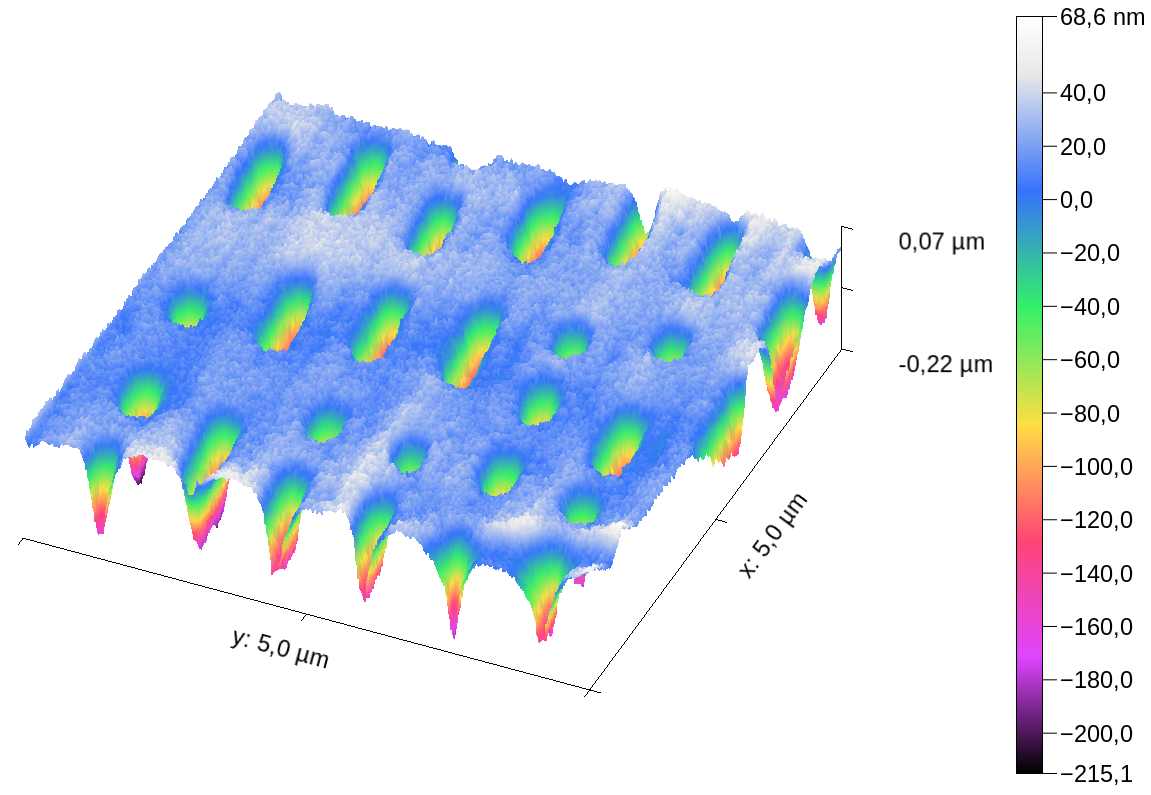
\includegraphics[width=\textwidth]{AFM_auswertung/dvd_3d.png}
	\caption{3D-AFM-Bild der DVD-Oberfl\"ache der Gr\"o{\ss}e $(5 \times 5) \, \upmu \text{m}^2$.}
	\label{abb:dvd_3d}
	\end{subfigure}
	~
	\begin{subfigure}[t]{0.5\textwidth}
	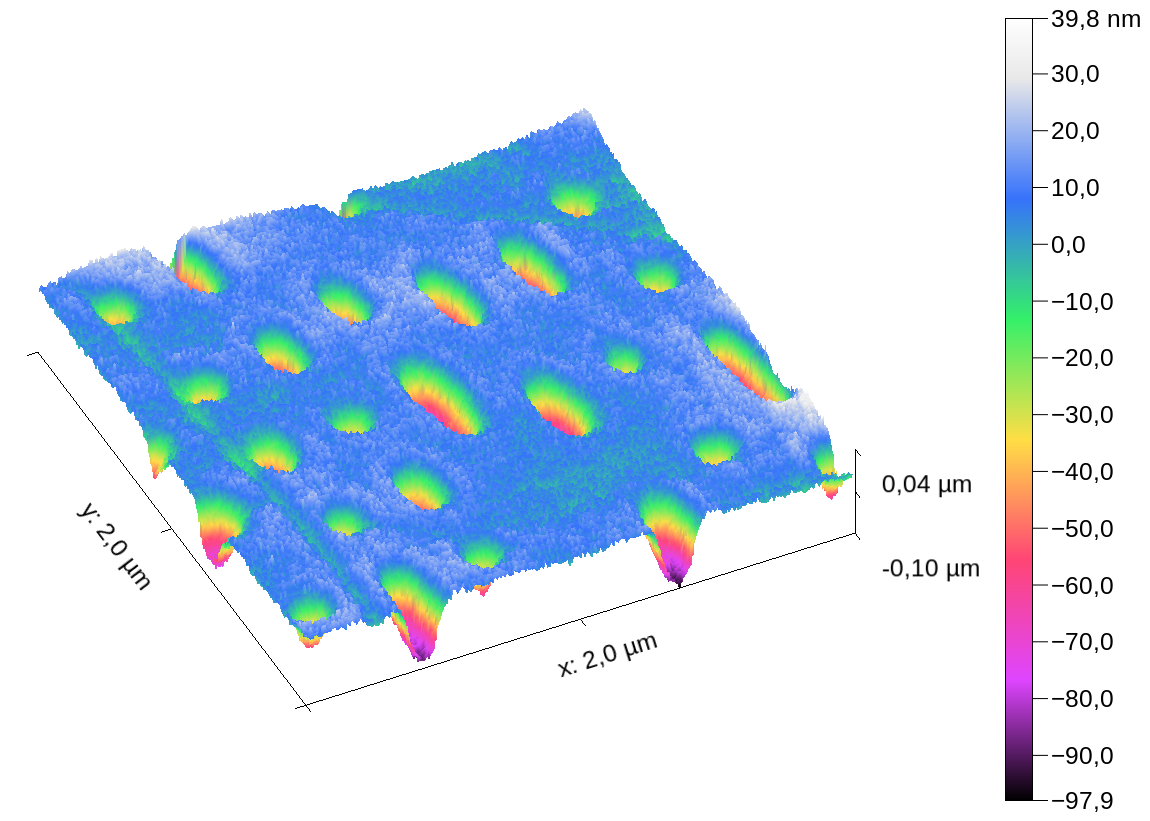
\includegraphics[width=\textwidth]{AFM_auswertung/bluray_3d.png}
	\caption{3D-AFM-Bild der Blu-ray-Oberfl\"ache der Gr\"o{\ss}e $(2 \times 2) \, \upmu \text{m}^2$.}
	\label{abb:br_3d}
	\end{subfigure}
\caption{Dargestellt sind hier in 3D die bearbeiteten AFM-Aufnahmen der drei zu untersuchenden Speichermedien.}
\label{abb:3d}
\end{figure}
Um die Speicherkapazit\"at der einzelnen Medien absch\"atzen zu k\"onnen, werden Gr\"o{\ss}e und Abst\"ande der Pits gemessen.
Dazu werden Pitbreite, minimale und maximale L\"ange der Pits sowie der Abstand zwischen zwei Pitspuren mit Hilfe von Gwyddion bestimmt.
In den Abbildung \ref{abb:cd_pitbreite} bis \ref{abb:cd_laenge} sind beispielhaft f\"ur die CD die AFM-Bilder hierzu abgebildet.
Die entsprechenden Aufnahmen der DVD und Blu-ray sind im Anhang zu finden (Abbildungen \ref{abb:DVD} und \ref{abb:BluRay}).
Die schwarzen unterschiedlich langen Streifen in den Bildern sind die Pits.% welche in die CD-Oberfl\"ache eingebrannt sind.
\begin{SCfigure}
\centering
	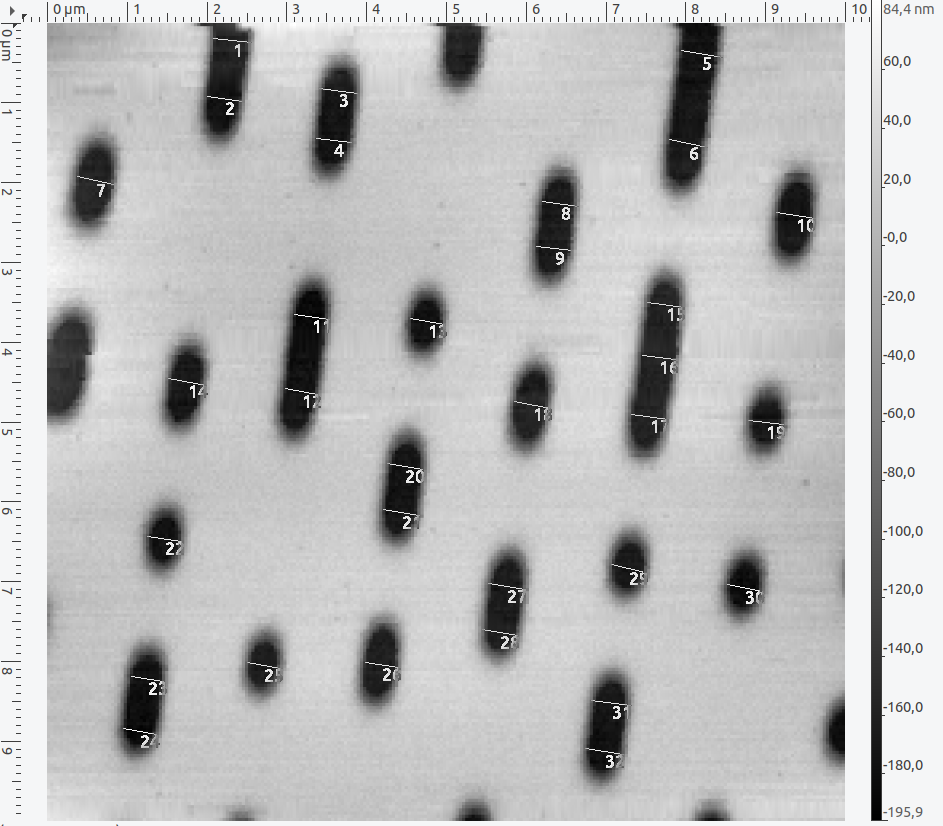
\includegraphics[width=0.5\textwidth]{AFM_auswertung/cd_breite.png}
	\caption{Um einen m\"oglichst aussagekr\"aftigen Werte der Pitbreite zu bestimmen, wird bei vielen Pits die Breite auch mehrfach vermessen und Pits, bei denen der Rand unscharft wird, werden nicht ber\"ucksichtigt.}
	\label{abb:cd_pitbreite}
\end{SCfigure}
%
\begin{SCfigure}
\centering
	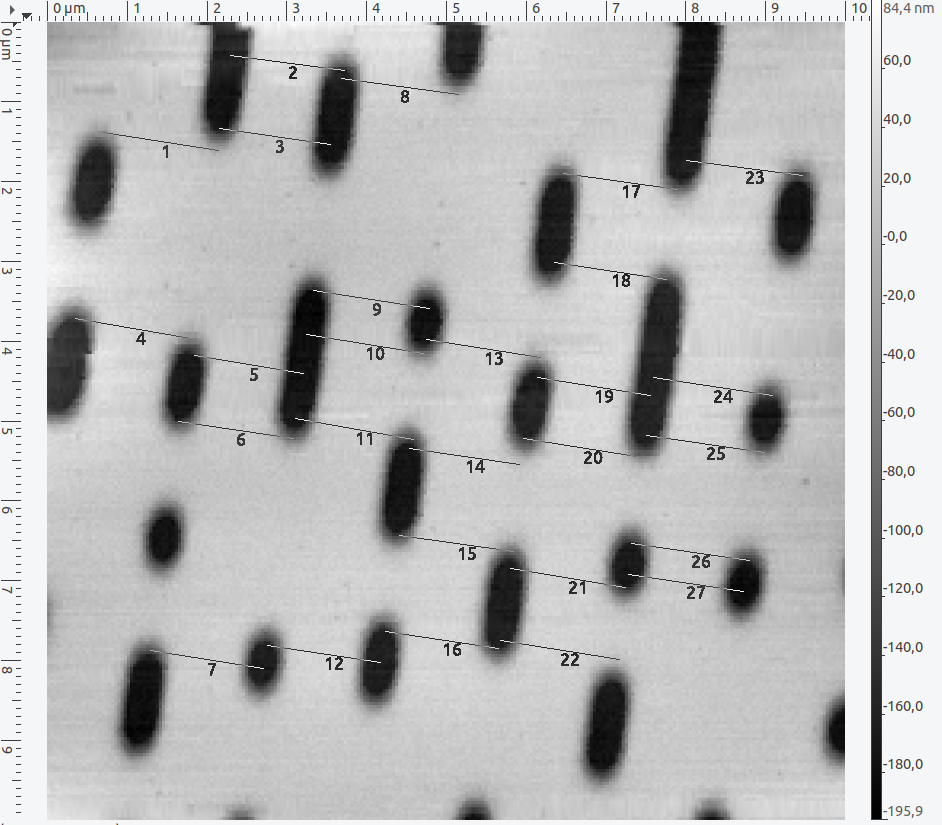
\includegraphics[width=0.5\textwidth]{AFM_auswertung/cd_abstand.png}
	\caption{Der Abstand zwischen den Pitspuren wird auch an so vielen Stellen wie m\"oglich gemessen, um ein gutes Messergebnis zu erzielen, da dieser Wert f\"ur die Absch\"atzung der Speichergr\"o{\ss}e wichtig wird.}
	\label{abb:cd_abstand}
\end{SCfigure}
%
\begin{SCfigure}
\centering
	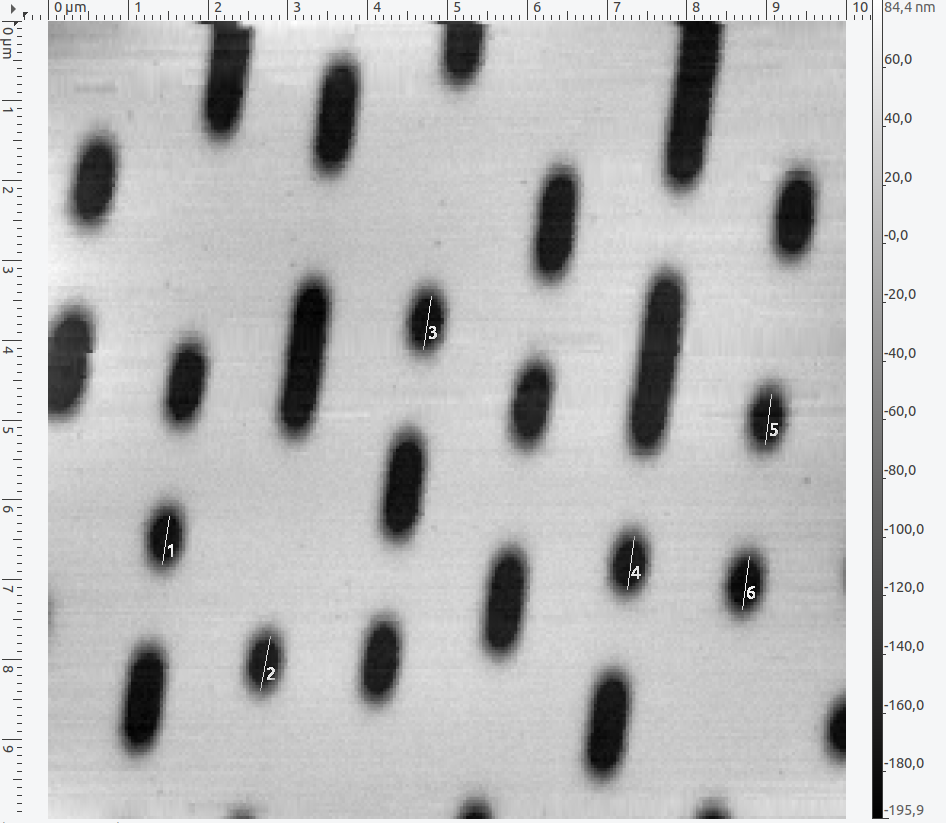
\includegraphics[width=0.5\textwidth]{AFM_auswertung/cd_Lmin.png}
	\caption{Die minimale Pitl\"ange kann hier von sechs, schon fast ovalf\"ormigen, Pits bestimmt werden.}
	\label{abb:cd_abstand}
\end{SCfigure}
%
\begin{SCfigure}
\centering
	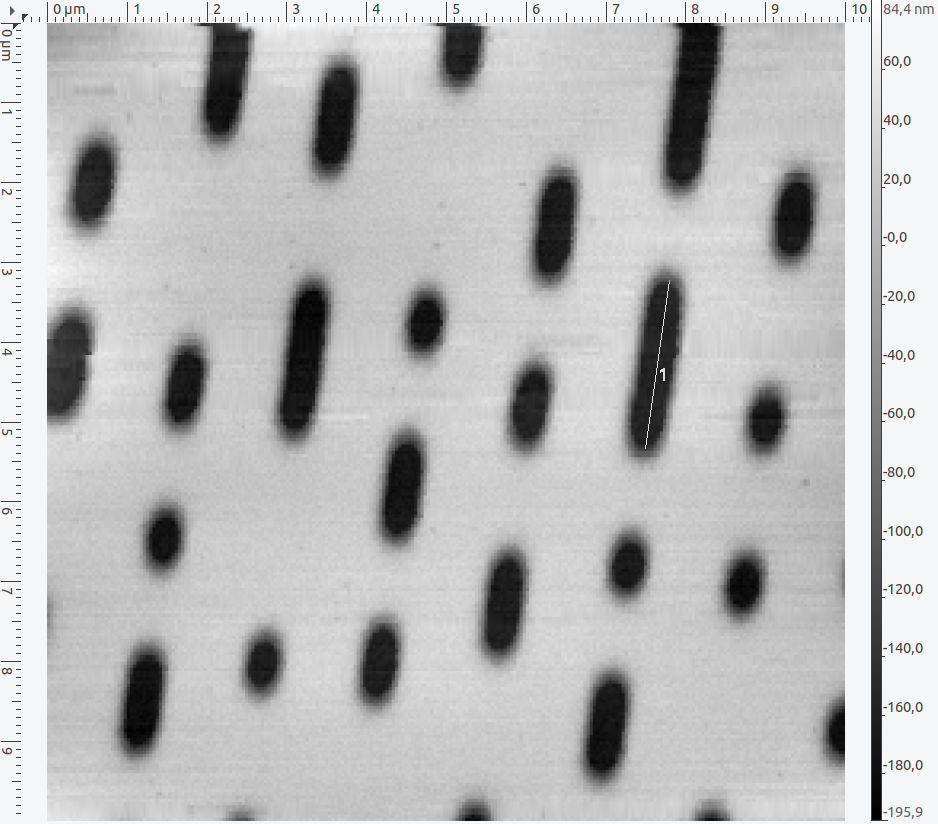
\includegraphics[width=0.5\textwidth]{AFM_auswertung/cd_Lmax.png}
	\caption{Die maximale Pitl\"ange kann hier nur von einem einzigen Pit bestimmt werden.}
	\label{abb:cd_laenge}
\end{SCfigure}
Bei allen Messungen der CD sowie DVD und Blu-ray werden m\"oglichst viele Pits vermessen.
Pits mit unklarem Rand werden dabei au{\ss}en vor gelassen.
\"Ahnliches gilt auch bei der Bestimmung der Pittiefen.
\begin{figure}[H]
\centering
	\begin{subfigure}[t]{0.45\textwidth}
	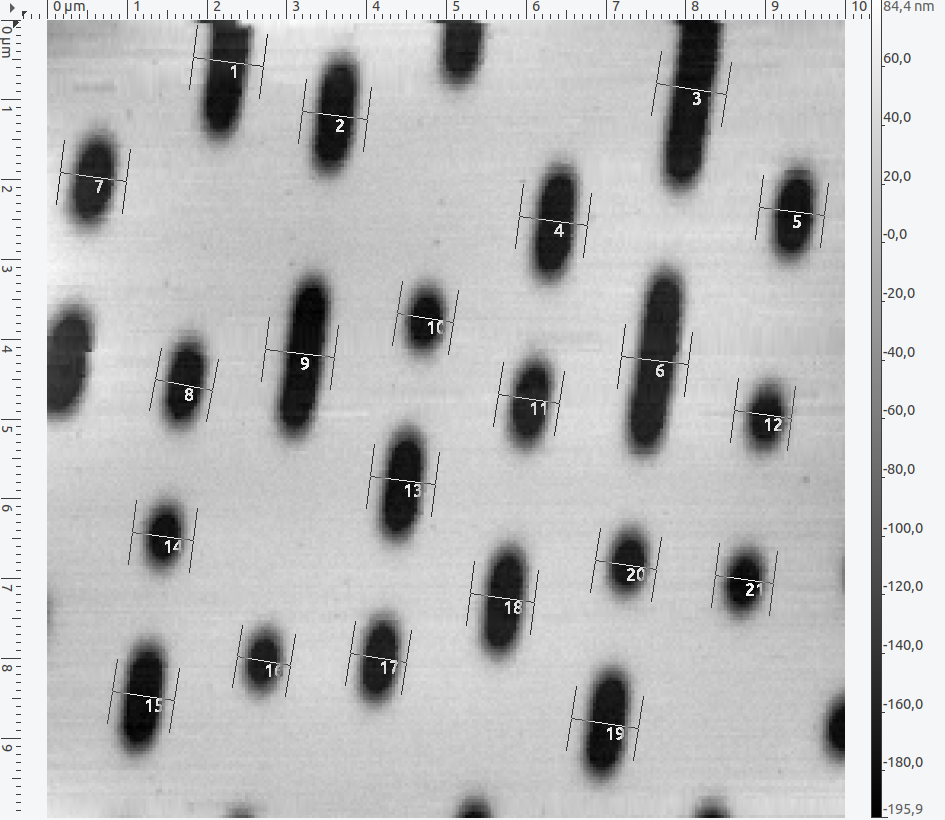
\includegraphics[height=7cm]{AFM_auswertung/cd_tiefe.png}
	\caption{}
	\end{subfigure}
	~
	\begin{subfigure}[t]{0.45\textwidth}
	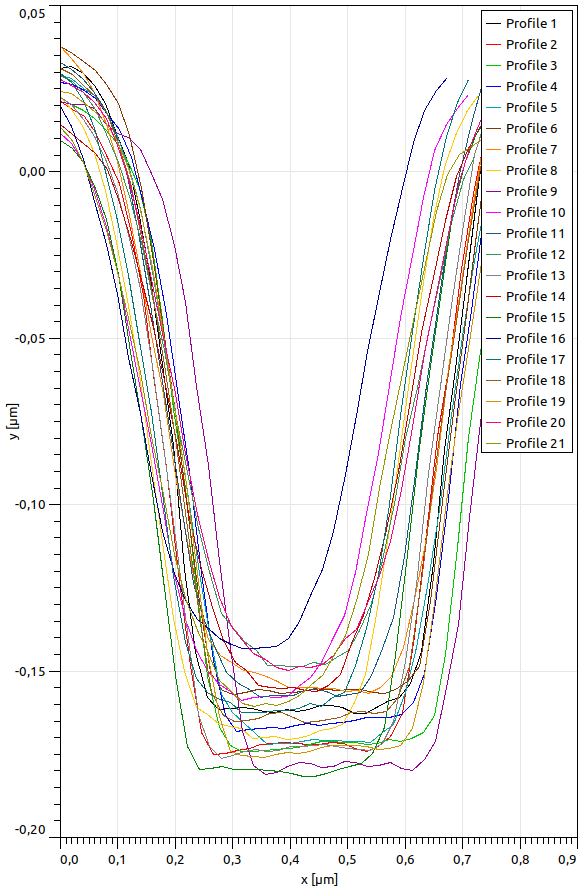
\includegraphics[height=10cm]{AFM_auswertung/cd_tiefe_grafik.png}
	\caption{}
	\label{abb:cd_tiefe}
	\end{subfigure}
\caption{Ermittlung der Pittiefen der untersuchten CD. In (a) ist die AFM-Aufname mit den markierten und nummerierten Bereichen zu sehen, welche f\"ur die Bestimmung der Pittiefen ausgewertet wurden. In (b) sind zu den nummerierten Bereichen die passenden Profil-Kurven gezeigt.}
\label{abb:pit_tiefe_cd}
\end{figure}
%
\begin{figure}[H]
\centering
	\begin{subfigure}[t]{0.45\textwidth}
	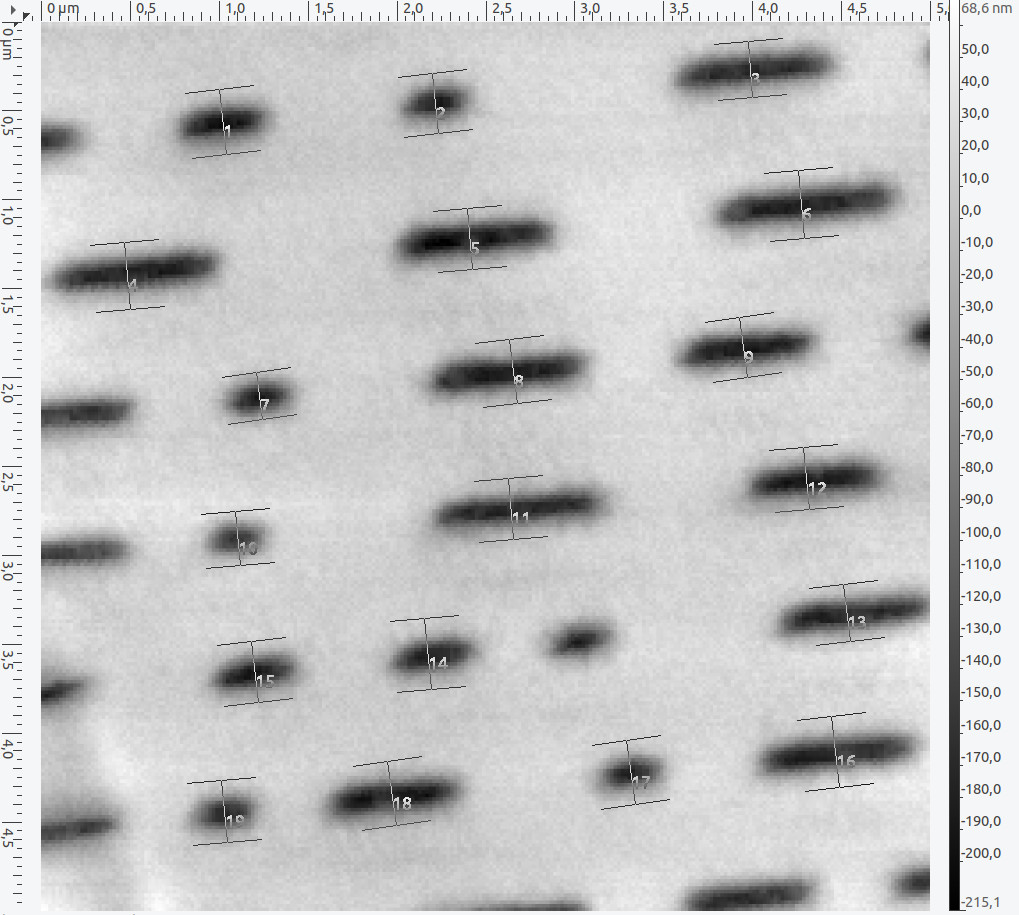
\includegraphics[height=7cm]{AFM_auswertung/dvd_tiefe.png}
	\caption{}
	\end{subfigure}
	~
	\begin{subfigure}[t]{0.45\textwidth}
	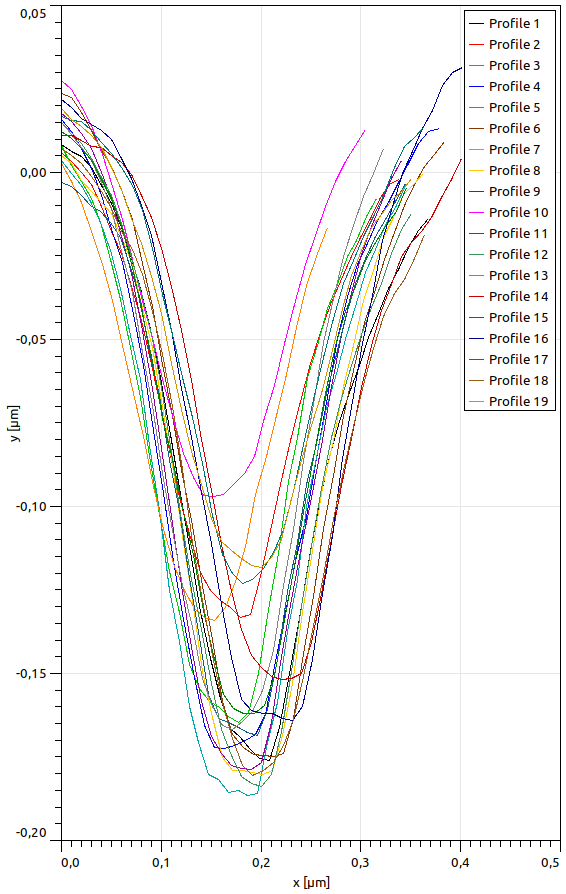
\includegraphics[height=10cm]{AFM_auswertung/dvd_tiefe_grafik.png}
	\caption{}
	\label{abb:dvd_tiefe}
	\end{subfigure}
\caption{Ermittlung der Pittiefen der untersuchten DVD. Wie schon in Abbildung \ref{abb:pit_tiefe_cd} ist in (a) die AFM-Aufname mit den markierten und nummerierten Bereichen zu sehen, welche f\"ur die Bestimmung der Pittiefen ausgewertet wurden. In (b) sind passend zu den nummerierten Bereichen die Profil-Kurven gezeigt.}
\label{abb:pit_tiefe_dvd}
\end{figure}
%
\begin{figure}[H]
\centering
	\begin{subfigure}[t]{0.45\textwidth}
	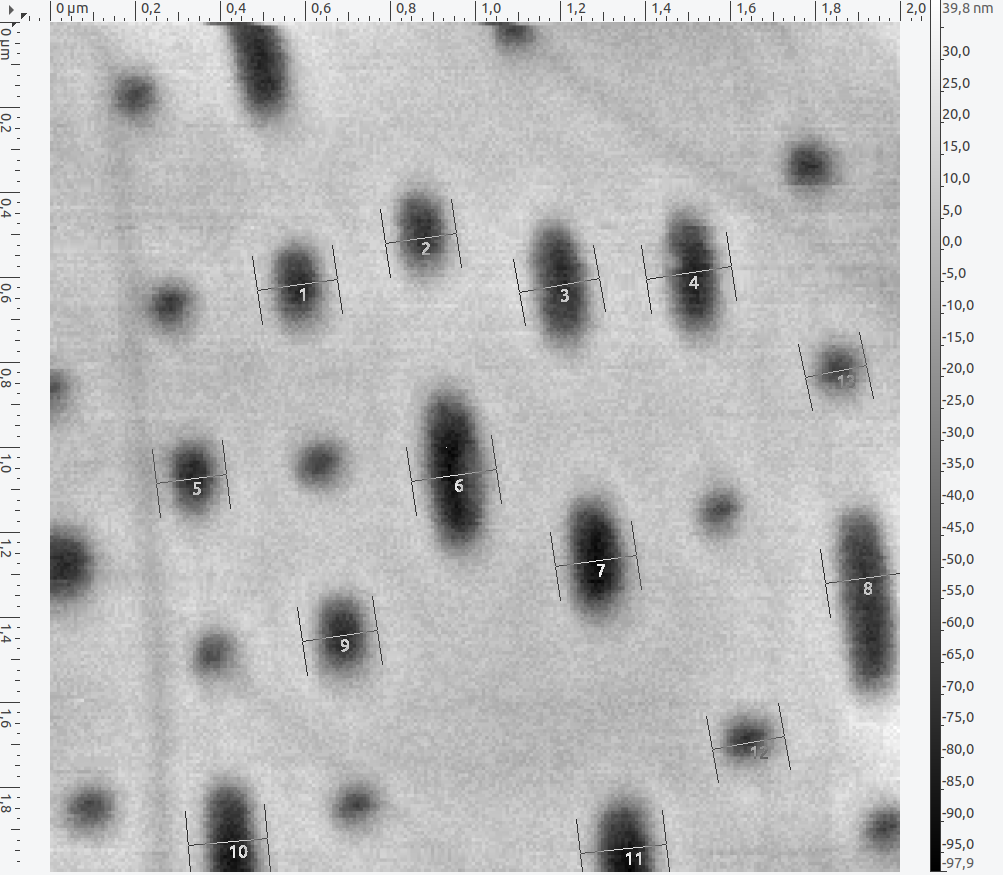
\includegraphics[height=7cm]{AFM_auswertung/bluray_tiefe.png}
	\caption{}
	\end{subfigure}
	~
	\begin{subfigure}[t]{0.45\textwidth}
	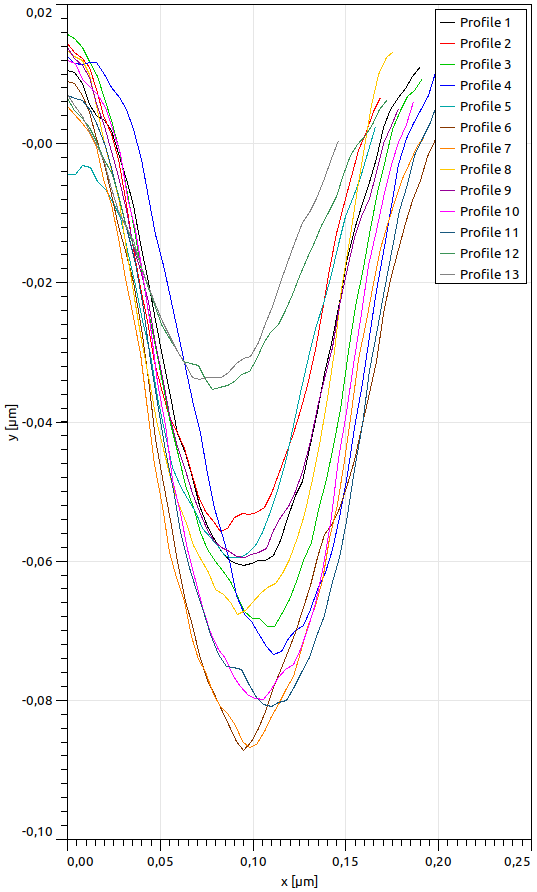
\includegraphics[height=10cm]{AFM_auswertung/bluray_tiefe_grafik.png}
	\caption{}
	\label{abb:br_tiefe}
	\end{subfigure}
\caption{In (a) ist die AFM-Aufname der Bluray-Oberfl\"ache mit den markierten und nummerierten Bereichen zu sehen, welche f\"ur die Ermittlung der Pittiefen ausgemessen werden. Und in (b) sind zu den nummerierten Bereichen die passenden Profil-Kurven gezeigt.}
\label{abb:pit_tiefe_br}
\end{figure}
In der folgenden Tabelle \ref{tab:auf2} sind alle berechneten Messwerte der untersuchten Speicher{\-}medien festgehalten.
Da bei der DVD und der Blu-ray jeweils nur bei einem Pit die maximale Pitl\"ange bestimmt wurde, besitzen diese Werte keinen Fehler.
Die Pittiefen der einzelnen Speichermedien wurden aus den Grafiken in den Abbildungen \ref{abb:cd_tiefe}, \ref{abb:dvd_tiefe} und \ref{abb:br_tiefe} abgesch\"atzt.
\begin{table}
	\centering
	\caption{Ermittelte Messwerte der Speichermedien.}
\begin{tabular}{|r|ccc|}
	\hline
	{} & {CD} & {DVD} & {Blueray} \\
	\hline
	Pitabstand / $\upmu \text{m}$ & $1,46 \pm 0,03$ & $0,78 \pm 0,01$ & $0,31 \pm 0,01$ \\
	Pitbreite	/ $\upmu \text{m}$ &	$0,45 \pm 0,02$ & $0,15 \pm 0,01$ & $0,10 \pm 0,01$ \\
	Minimale Pitlänge / $\upmu \text{m}$ & $0,66 \pm 0,03$ & $0,30 \pm 0,02$ & $0,10 \pm 0,01$ \\
	Maximale Pitlänge / $\upmu \text{m}$ & 2,13 & $0,86 \pm 0,02$ & 0,44 \\
	Pittiefe / $\upmu \text{m}$ & 0,16 & 0,17 & 0,07 \\
	\hline
\end{tabular}
\label{tab:auf2}
\end{table}
Zum Abschluss wird die Speicherkapazit\"at einer CD anhand der gemessenen Daten abgesch\"atzt.
Ausgehend von einer CD mit Innenradius $r_{\text{i}} = 2,25 \, \text{cm}$ und Au{\ss}enradius $r_{\text{a}} = 5,9 \, \text{cm}$, ergibt sich eine verf\"ugbare Speicherfl\"ache von:
\begin{align*}
	\text{Speicherfl\"ache:} \, A = \pi \cdot \left( r_{\text{a}}^2 - r_{\text{i}}^2 \right) = 0,0093455 \, \text{m}^2
\end{align*}
Da die Daten auf einer CD spiralf\"ormig gespeichert werden, muss nun durch den ermittelten Pitabstand dividiert werden, um die Gesamtspurl\"ange zu ermitteln.
So ergibt sich folglich:
\begin{align*}
	\text{Spurl\"ange} \, = 6405,38 \, \text{m}
\end{align*}
Die minimale Pitl\"ange entspricht einer Bit-Folge von "1001".
So kann von der Spurl\"ange auf die maximale Anzahl an Bit geschlossen werden, die auf eine CD passen.
Nach der Eight-to-Fourteen-Methode ergeben $17$ Bit zusammen einen Byte.
Es passen demnach maximal $2,298 \,$GB auf die untersuchte CD.
Zu beachten ist jedoch, dass von den $17$ Bit nur $8$ Bit zum Speichern von Daten dienen.
Die restlichen Bit dienen lediglich zum Trennen  der Bits und besseren Auslesen der gespeicherten Daten.
So bleiben noch $1081,17 \,$MB Speicherkapazit\"at auf der CD \"ubrig.

\subsection{Kraft-Abstandskurven}
In der letzten Versuchsreihe werden f\"ur drei Materialproben die Kraft-Abstandskurven aufgenommen.
Diese sind in den Abbildungen \ref{abb:edelstahl} und \ref{abb:teflonTiN} dargestellt.
\begin{figure}[hbtp]
	\centering
	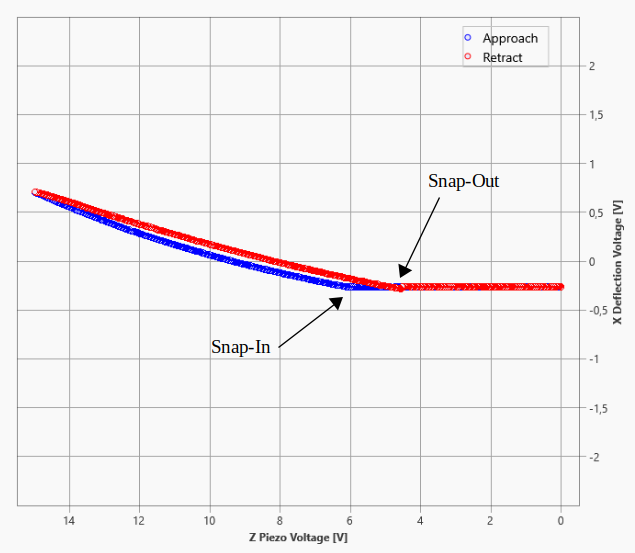
\includegraphics[width=0.45\textwidth]{AFM_auswertung/edelstahl_pfeile.png}
	\caption{Die Kraft-Abstandskurve der Edelstahl-Probe.}
\label{abb:edelstahl}
\end{figure}
Aus den Graphen werden die 'Snap-In'- und 'Snap-Out'-Bereiche abgelesen.
Beispielhaft sind diese Bereiche in Abbildung \ref{abb:edelstahl} eingezeichnet.
\begin{figure}[H]
\centering
	\begin{subfigure}[t]{0.45\textwidth}
	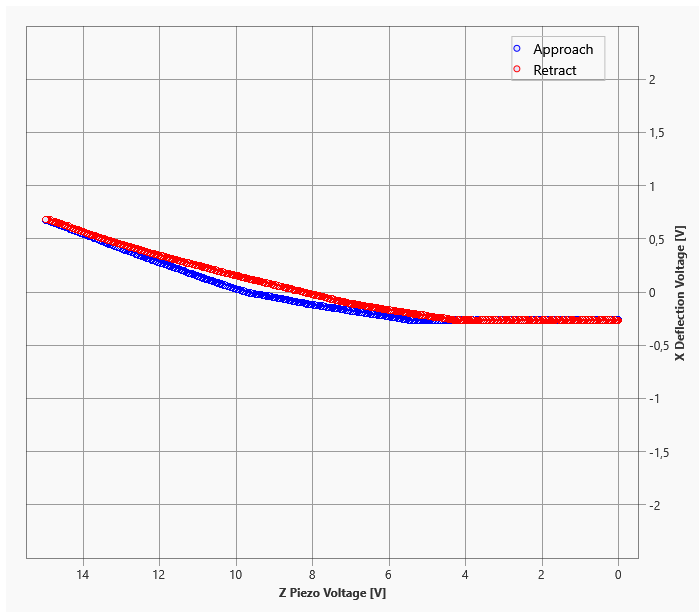
\includegraphics[width=\textwidth]{AFM_auswertung/teflon_kurve.png}
	\caption{Teflon-Probe.}
	\label{abb:teflon}
	\end{subfigure}
	~
	\begin{subfigure}[t]{0.45\textwidth}
	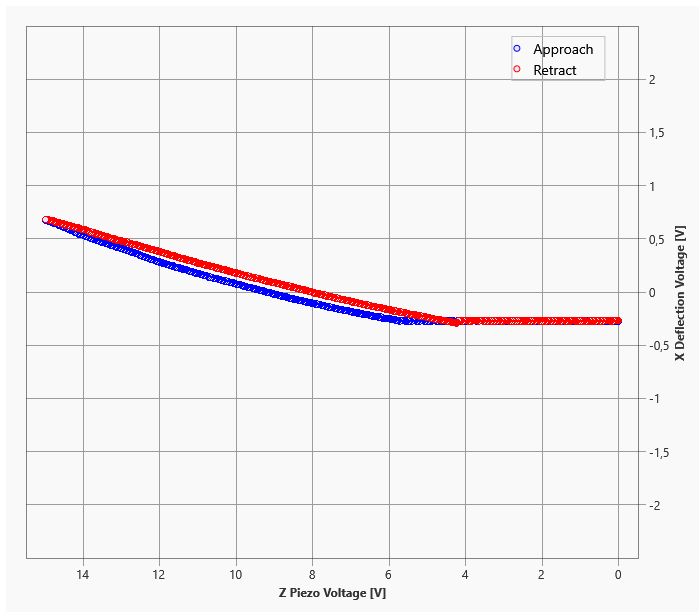
\includegraphics[width=\textwidth]{AFM_auswertung/TiN_kurve.png}
	\caption{TiN-Schicht-Probe.}
	\end{subfigure}
\caption{Die aufgenommenen Kraft-Abstandskurven der Teflon- und TiN-Probe.}
\label{abb:teflonTiN}
\end{figure}
Um von den Kraft-Abstandskurven auf die maximale Adh\"asionskraft zu schlie{\ss}en wird zun\"achst der Höhenunterschied $\Delta z$ des z-Piezoelements mit Formel (\ref{equ:deltaZ}) bestimmt.
\begin{align}
	\Delta z = \left\vert z_{\text{in}} - z_{\text{out}} \right\vert
\label{equ:deltaZ}
\end{align}
Mit Gleichung (\ref{equ:AdhKraft}) kann nun die maximale Adh\"asionskraft berechnet werden.
Wobei $k_{\text{cantilever}} = 0,2 \, \frac{N}{m}$ betr\"agt und die Federkonstante des Cantilevers wiedergibt.
Zu beachten ist noch, dass das z-Piezo-Element bei einer Maximalspannung von $75 \, V$ um $20 \, \mu m$ ausgelenkt wird.
Mittels Dreisatz wird der Höhenunterschied $\Delta z$ so von Volt in Meter umgerechnet.
\begin{align}
	F_{\text{Adh\"a}} = \Delta z \cdot k_{\text{cantilever}}
\label{equ:AdhKraft}
\end{align}
Diese Rechnung wird f\"ur alle drei untersuchten Materialproben vorgenommen.
Die Messergebnisse sind in Tabelle \ref{tab:auf3} notiert.
\begin{table}
	\centering
	\caption{Ermittelte und berechnete Daten zur Bestimmund der maximale Adhäsionskraft von Edelstahl, Tefon und der TiN-Schicht Probe.}
\begin{tabular}{|r|cccc|}
	\hline
	{Probe} & {$U_{\text{snap-in}}$} / V & {$U_{\text{snap-out}}$} / V & $\Delta z$ / V & {$F_{\text{Adh\"a}}$} / N \\
	\hline
	Edelstahl & 6,188 & 4,556 & 1,632 & $8,704 \cdot 10^{-8}$ \\
	Teflon	& 5,569 & 4,406 & 1,163 & $6,203 \cdot 10^{-8}$ \\
	TiN-Schicht & 5,981 & 4,219 & 1,762 & $9,397 \cdot 10^{-8}$ \\
	\hline
\end{tabular}
\label{tab:auf3}
\end{table}
Abschlie{\ss}end wird noch der Elastizitätsmodul der Teflon-Probe abgesch\"atzt.
Hierf\"ur wird die Auslenkung von Teflon mit der h\"arteren Edelstahlprobe verglichen und die Eindringtiefe $d$ der Cantileverspitze in die Teflonprobe bestimmt.
Dieser Vergleich ist in Abbildung \ref{abb:3d} dargestellt.
Der Abstand der Teflonkurve zur Edelstahlprobe bei maximaler Auslenkung des Cantilevers beschreibt die Eindringtiefe $d$ der Cantileverspitze.
Die effektive Auslenkung des Cantilevers $\delta$ kann mit $\delta = z_p - d$ berechnet werden.
Wobei $z_p$ der Auslenkung des Probentisches, dem Verfahrweg, entspricht.
\begin{figure}[hbtp]
	\centering
	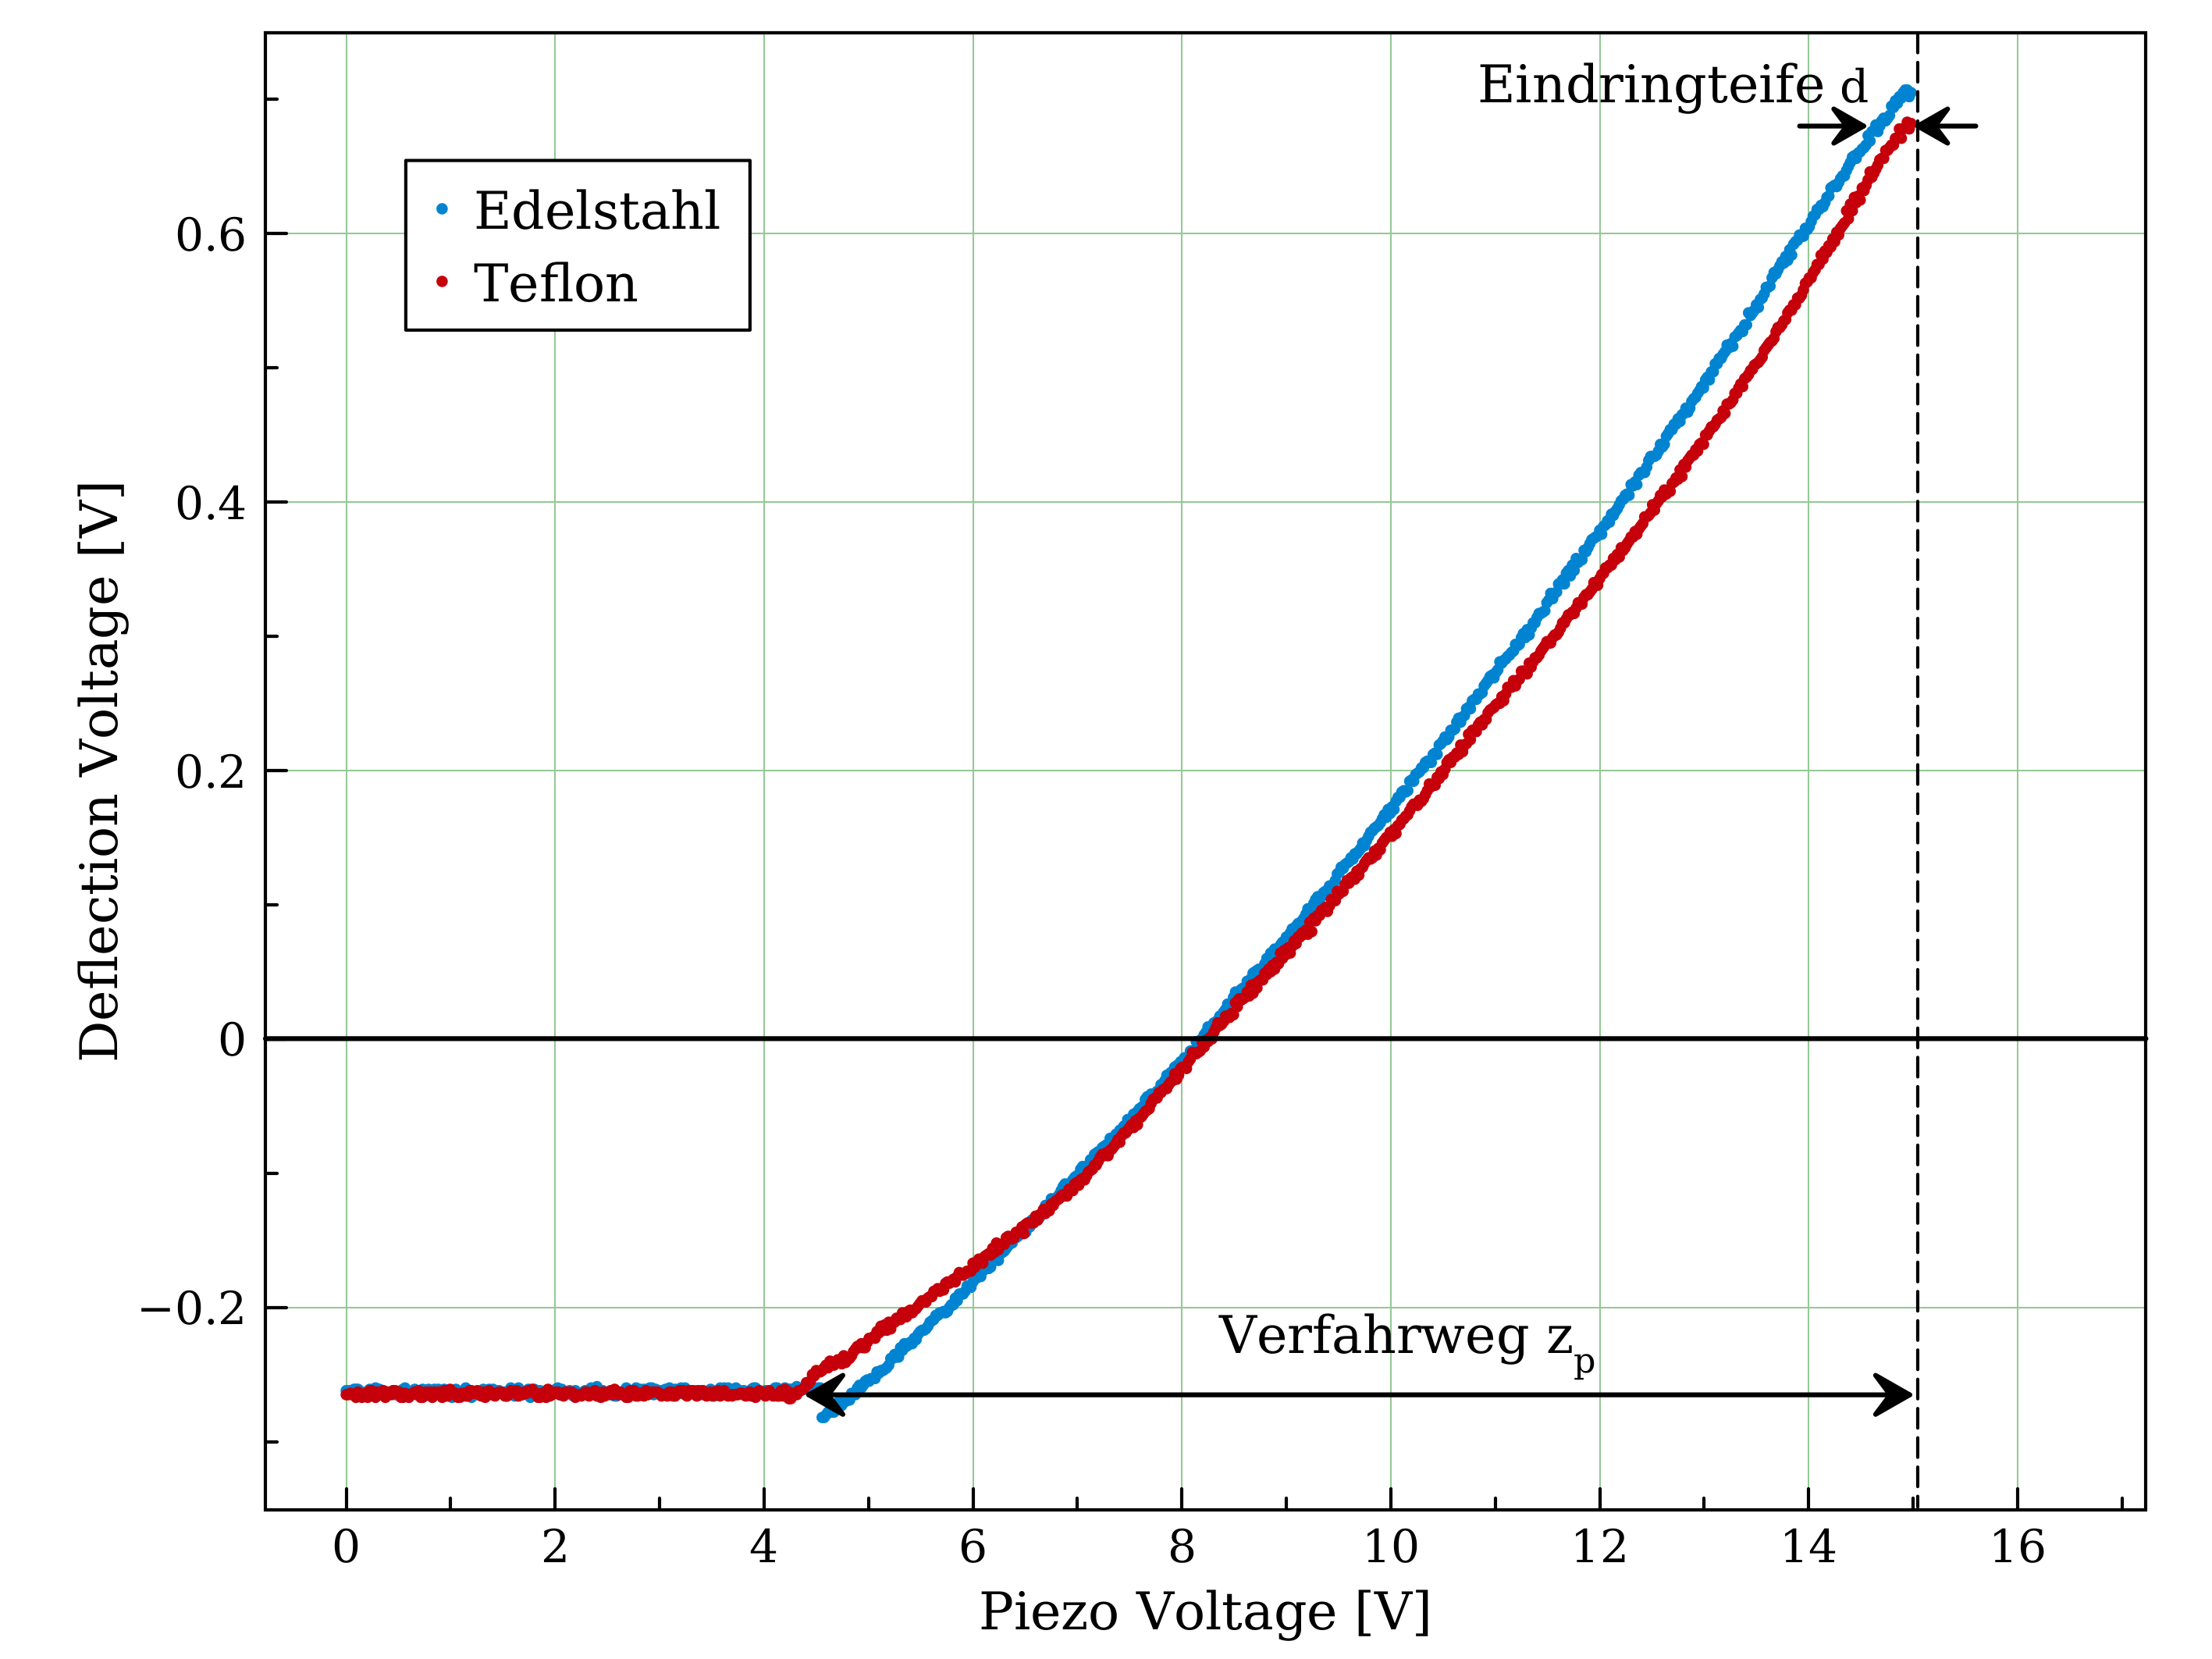
\includegraphics[width=0.45\textwidth]{AFM_auswertung/elastizitaet.png}
	\caption{Vergleich der Annäherungskurven des Cantilevers an die Teflonprobe und die Edelstahlprobe. Eingezeichnet sind die Eindringtiefe d und der Verfahrweg $z_p$.}
	\label{abb:auf3c}
\end{figure}
Mittels der Daten aus Abbildung \ref{abb:3d} und Gleichung (\ref{equ:Elastizitaet}) wird der Elastizitätsmodul von Teflon berechnet.
\begin{align}
	E = \frac{k_{\text{cantilever}} \cdot \delta \cdot \pi \cdot \left( 1 - \upsilon^2 \right)}{2 tan(\alpha) \cdot d^2}
\label{equ:Elastizitaet}
\end{align}
Hierbei gibt $\alpha$ den Öffnungswinkel der pyramidenförmigen Cantileverspitze an, dieser betr\"agt f\"ur den hier verwendeten Cantilever $10^{\circ}$.
Die Poissonzahl von Teflon wird mit $\upsilon = 0,46$ angenommen.
Es folgt:
\begin{align*}
	E_{\text{Teflon}} = 474,83 \, \text{MPa}
\end{align*}
